\section{Applications}
\label{sec:apps}

Each application example is a notebook in the online material: We could have one
analysis as Python scripts instead of notebook in the online material. At the
start of this section, point to gammapy-paper repo on Github and say that
there’s a Binder where people can try the examples online.

TODO: mention other application examples (joint Crab paper, HESS validation
paper, HGPS, ...) here or in a subsection "other applications" at the end of
this section?

\subsection{Source detection}
\label{apps:detect}

See Figure~\ref{fig:fermi-ts-image}.

Ref: \citep{Stewart2009}

\begin{figure*}[t]
\centering
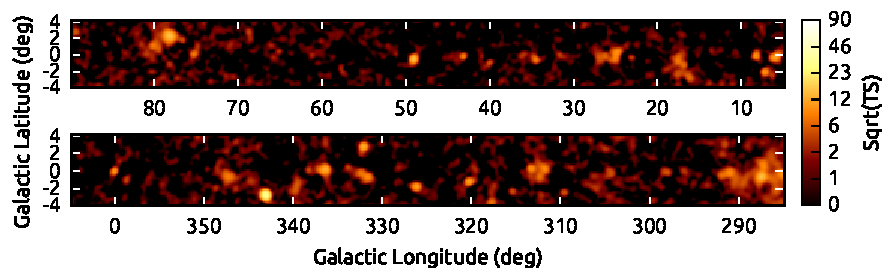
\includegraphics[width=1.\textwidth]{figures/gammapy-fermi-ts-image}
\caption{
Gammapy application example: A \textit{Fermi} survey TS map of the inner
Galactic plane region.
}
\label{fig:fermi-ts-image}
\end{figure*}

\begin{figure*}[t]
\centering
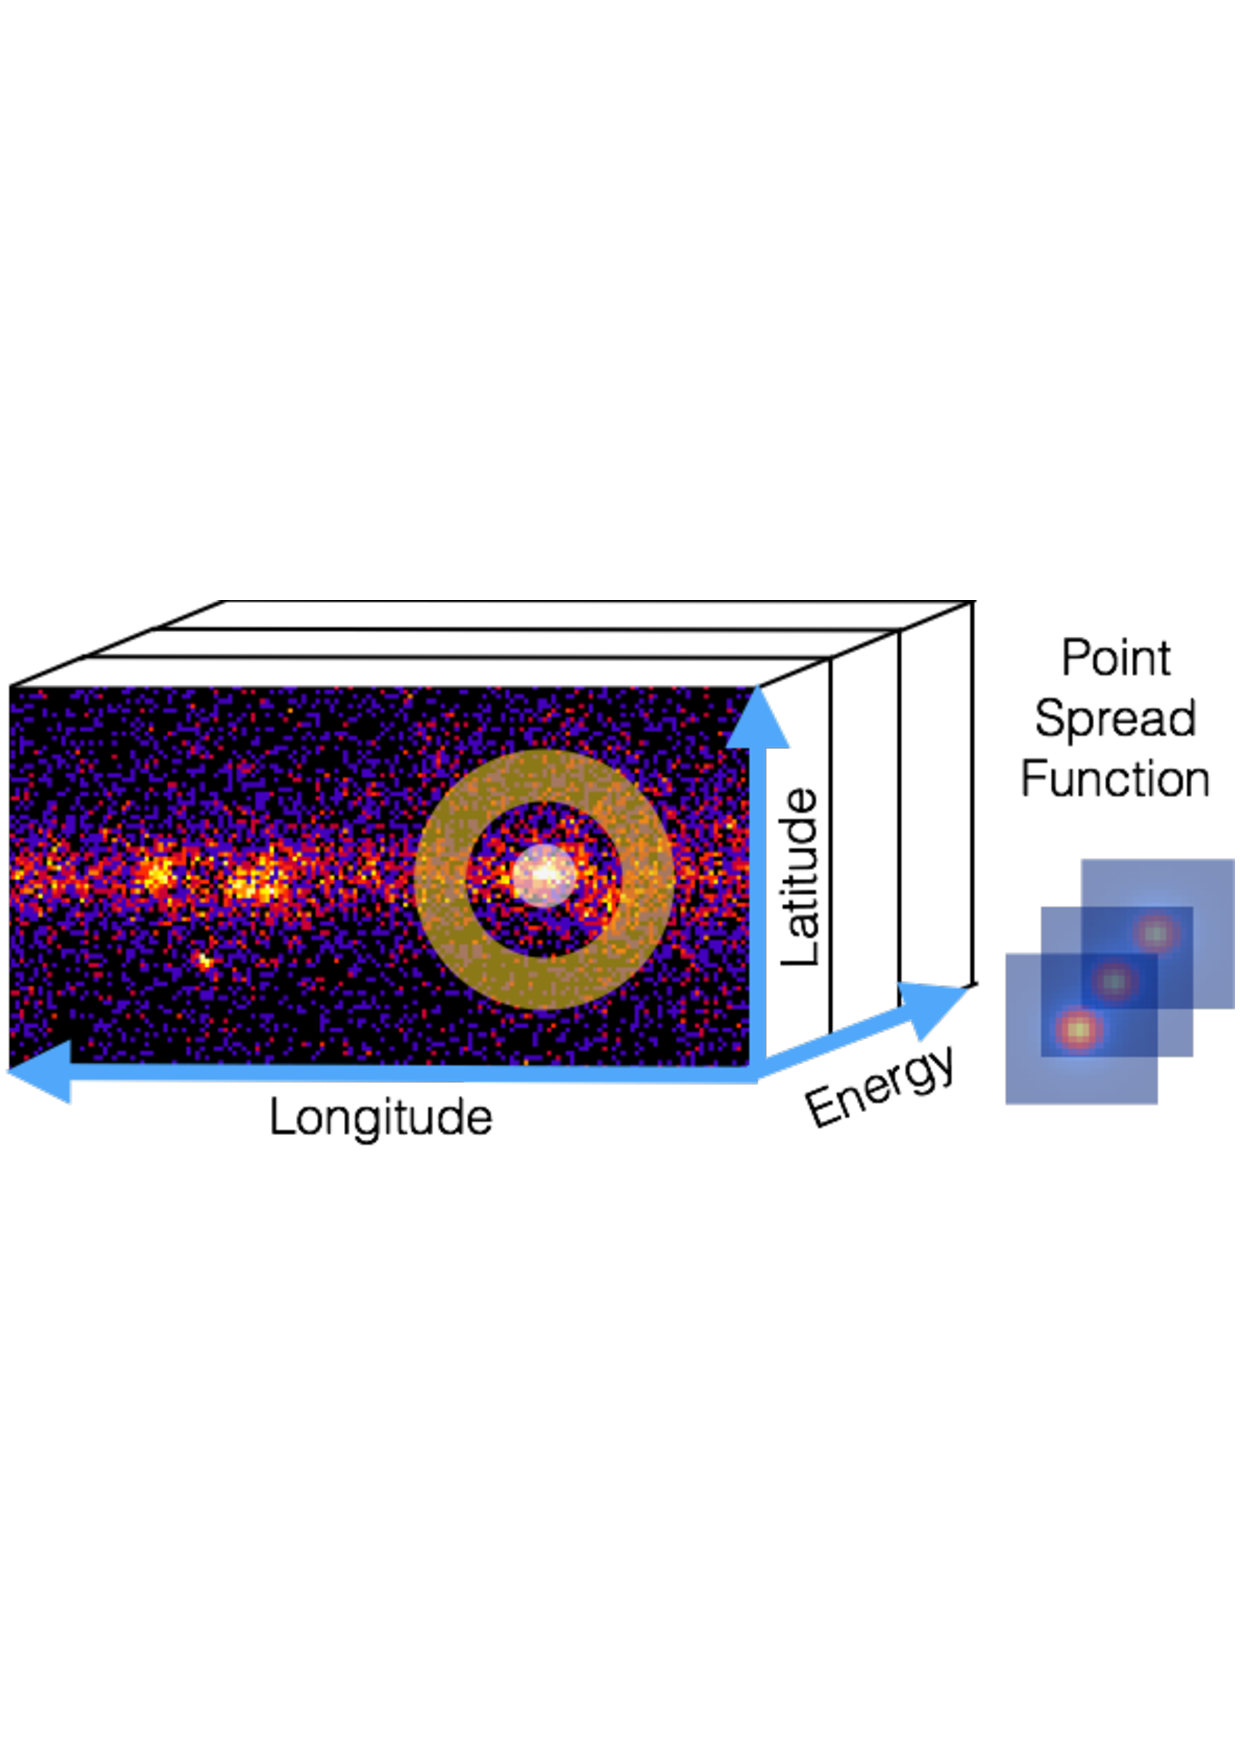
\includegraphics[width=0.8\textwidth]{figures/gammapy-cube-analysis}
\caption{
Gammapy data model illustration. Binned analysis of lon-lat-energy cube data is
supported via joint likelihood analysis of one image per energy bin.
On-off-region based spectral analysis is supported as well.
}
\label{fig:data-model}
\end{figure*}

\subsection{Multi instrument analysis}

